\section{Performance Evaluation and Discussion \label{sec:evaluation}}

This section presents the evaluation results on the \gls{raw} performance predication accuracy of our surrogate model. First, the  convergence of the training process is evaluated. Subsequently, the accuracy of the surrogate model for the design space and the \textcolor{red}{extrapolated} design space are evaluated respectively. Finally, the optimal \gls{raw} configurations are discussed. As mentioned in Section \ref{subsec:para_design}, there are a number of coverage and packet size ranges that can lead to the same average transmission time. For the \textcolor{red}{limited} design space, the average transmission time is only represented by distance and packet size range used during the training process. While in the extrapolated design space, there is no such limitation.

All evaluations are performed using our previously developed
IEEE 802.11ah ns-3 module \cite{WNS32016}, and we consider the same IEEE~802.11ah scenario as described in Section \ref{subsec:80211ah_raw}. The same default PHY and MAC layer parameters are used as shown in Table \ref{tab:ns3 parameters}.

%\subsection{Exhaustive Search Model}
%[Probably too hard to run all these experiments]

\subsection{Training convergence}
%Cross validation score evolution, stopping criterion, ...
\begin{figure}[t]
  \centering
  \includegraphics[width=0.75\columnwidth]{figures/throughput-cv}
  \caption{Cross validation score of the surrogate model as a function of the number of training samples. \label{fig:sumo-iteraton}}
\end{figure}

In this section we evaluate the training convergence of
the surrogate model. The cross validation score is widely used to measure the accuracy of the resulting model, a low score signifies the high accuracy of the model, and vice versa. Figure~\ref{fig:sumo-iteraton} demonstrates the 10-fold cross validation score of the model as a function of the number of training samples used, each iteration uses 10 extra samples for training.  %\textcolor{red}{explains the cross validation either in this section or modeling section}.
It clearly shows that at first, SUMO is trying to learn the behavior of the networks with cross validation score going up and down, while from 1360 samples onward, the cross validation score continually decreases until 5400 samples used for training, reaches \textcolor{red}{0.10x}. Then the cross validation score remains almost constant, signifying that the training process has converged.  Training of the model stopped after 5600 samples as it satisfied the stop conditions, i.e., 10 consecutive cross-validation scores lower than or equal to $0.10$ (2 digits of precision). \textcolor{red}{This comes down to about 
about xx(5600/425799?) of the reduced parameter space (i.e., xx), as listed in table \ref{tab:sumo parameters}, from which samples were drawn during training, and xx(5600/??) of all data points in the design space (i.e., xx), in which the step size is \textcolor{red}{1} and the results for data points outside the reduced parameter space are obtained via interpolation by the Kriging  model.}


%This comes down to about xx(5600/??) of all data points in the input space (i.e., xx), and about xx(5600/425799?) of the reduced data space (i.e., xx) from which samples were drawn during training.



\subsection{Design space experiments}
% \begin{figure*}[t]
%     \centering
%     \subfloat[all \label{fig:throughput-alpha-0}]{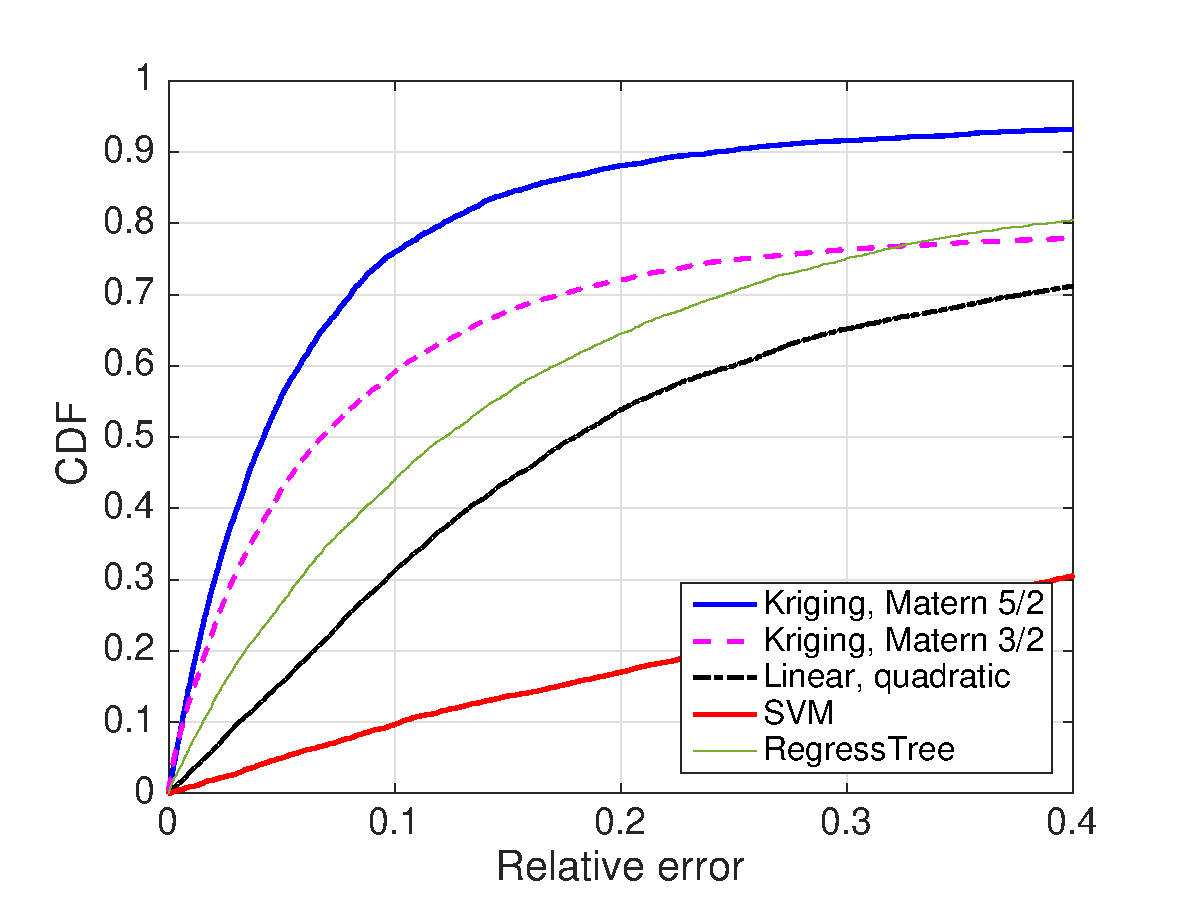
\includegraphics[width=0.30\textwidth]{figures/all}}
%     \subfloat[1\_50 \label{fig:delay-alpha-0}]{\includegraphics[width=0.30\textwidth]{figures/1_50}}
%     \subfloat[1\_10 \label{fig:delay-alpha-0}]{\includegraphics[width=0.30\textwidth]{figures/1_10}}
%   \caption{Comparison of different regression models. \label{fig:regress-models}}
% \end{figure*}


\begin{figure}[t]
    \centering
{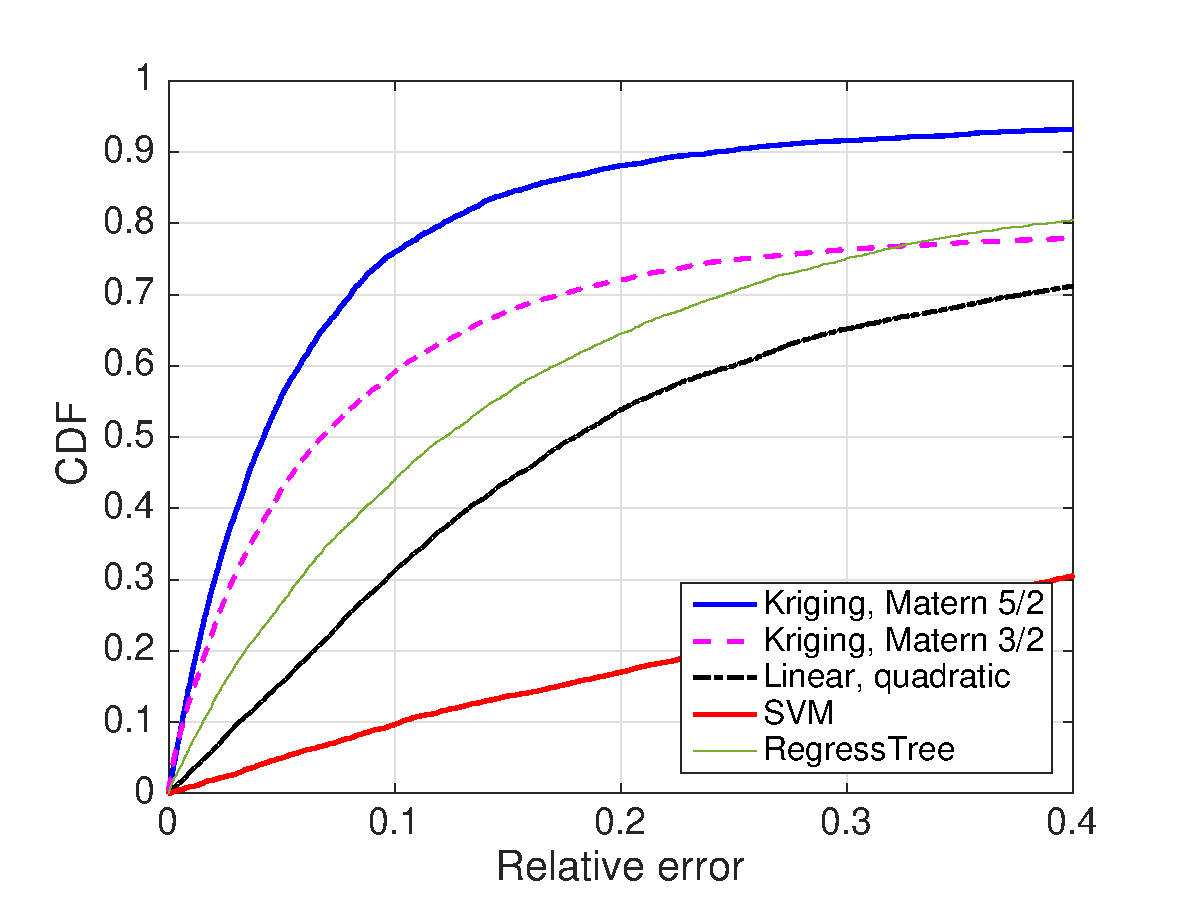
\includegraphics[width=0.8\columnwidth]{figures/all}}
  \caption{Performance comparison between different regression models and simulation results for 6000 random test data
points. \label{fig:regress-models}}
\end{figure}





% \begin{figure}[t]
%     \centering
% {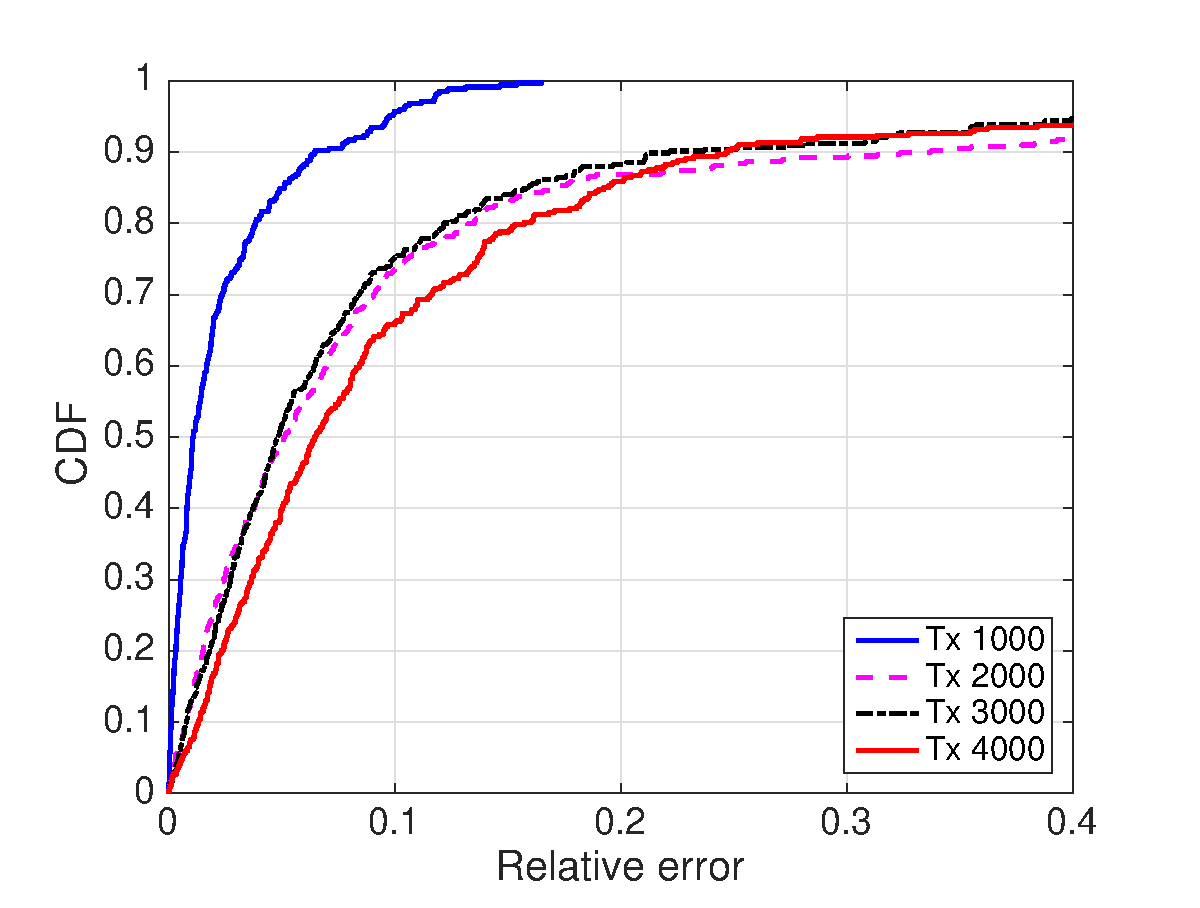
\includegraphics[width=0.8\columnwidth]{figures/cdf_f1000_t4000}}
%   \caption{Comparison of different regression models. \label{fig:regress-models-a}}
% \end{figure}



% \begin{figure*}[t]
%     \centering
%     \subfloat[Relative error $>=$ 0 \label{fig:delay-alpha-0}]{\includegraphics[width=0.33\textwidth]{figures/scatter_results-error-GPR5020-opti-all-sort_L0}}
%     \subfloat[Relative error $>=$ 0.1  \label{fig:delay-alpha-0}]{\includegraphics[width=0.33\textwidth]{figures/scatter_results-error-GPR5020-opti-all-sort_L0_1}}
%      \subfloat[Relative error $>=$ 0.2  \label{fig:delay-alpha-0}]{\includegraphics[width=0.33\textwidth]{figures/scatter_results-error-GPR5020-opti-all-sort_L0_2}}
%   \caption{Scatter plot. \label{fig:scatter-plot}}
% \end{figure*}

% \begin{figure*}[t]
%     \centering
%     \subfloat[Surrogate model prediction vs. simulation results \label{fig:scatter_all}]{\includegraphics[width=0.45\textwidth]{figures/scatter_full}}
%     \subfloat[Relative error  \label{fig:full_design_error}]{\includegraphics[width=0.45\textwidth]{figures/full_design_error}}
%   \caption{Comparison between the simulation results and surrogate model's prediction for the test data points, in terms of average packet receiving rate \label{fig:scatter-plot}}
% \end{figure*}


\begin{figure*}[t]
    \centering
    \subfloat[Surrogate model prediction vs. simulation results \label{fig:scatter_all}]{\includegraphics[width=0.33\textwidth]{figures/scatter_full}}
    \subfloat[Relative error for all packet receiving rate \label{fig:full_design_error}]{\includegraphics[width=0.33\textwidth]{figures/full_design_error_all}}
     \subfloat[Relative error for all packet receiving rate larger than 50 \textcolor{red}{pps}. \label{fig:full_design_error}]{\includegraphics[width=0.33\textwidth]{figures/full_design_error_L50}}
  \caption{Comparison between the simulation results and surrogate model's prediction for the test data points, in terms of average packet receiving rate \label{fig:scatter-plot}}
\end{figure*}

\begin{figure*}[t]
    \centering
    \subfloat[Tx 1000 us  \label{fig:scatter_ana_tx1000}]{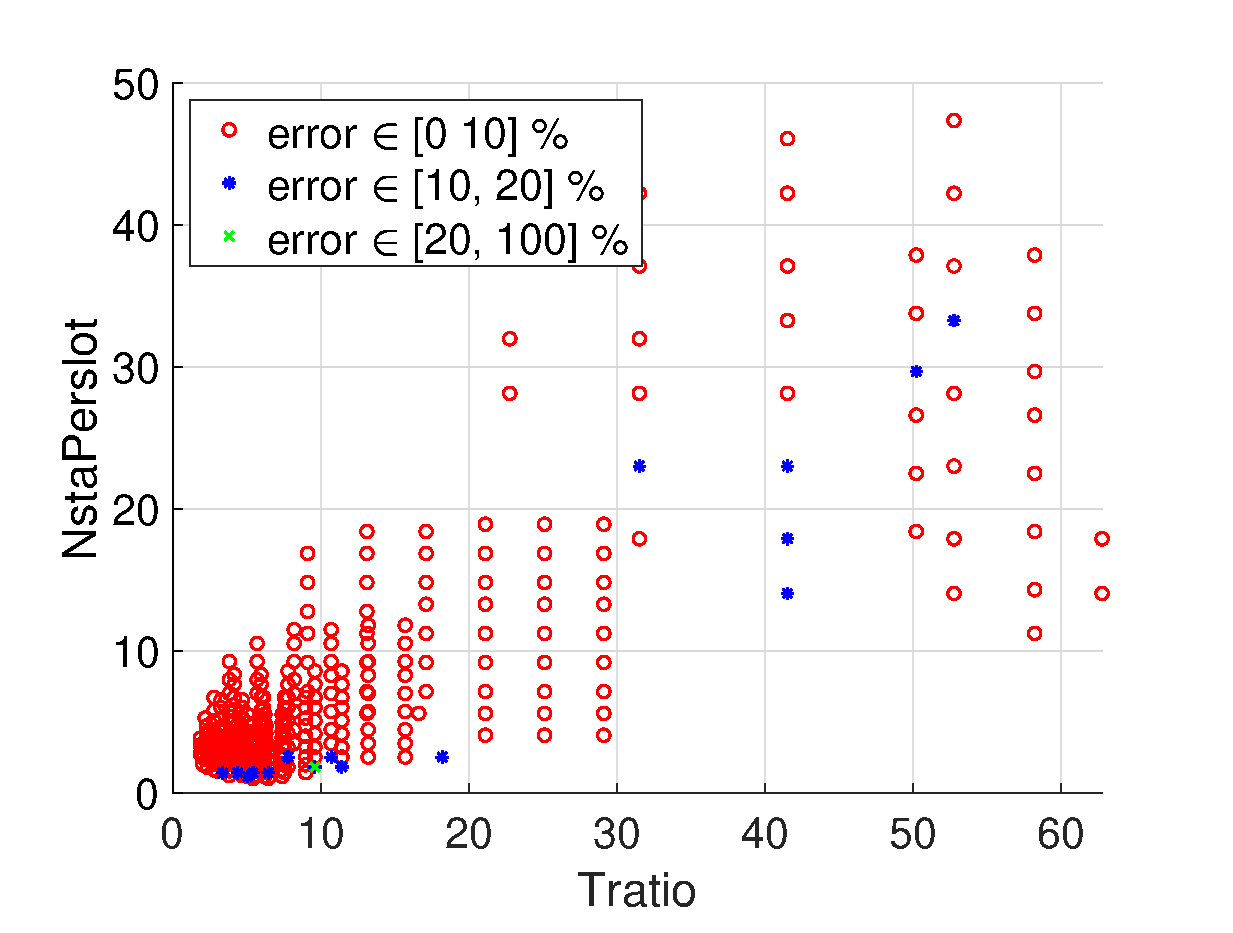
\includegraphics[width=0.33\textwidth]{figures/nstaPerSlot_Tratio_scatter_tx1000}}
    \subfloat[Tx 3000 us \label{fig:scatter_ana_tx3000}]{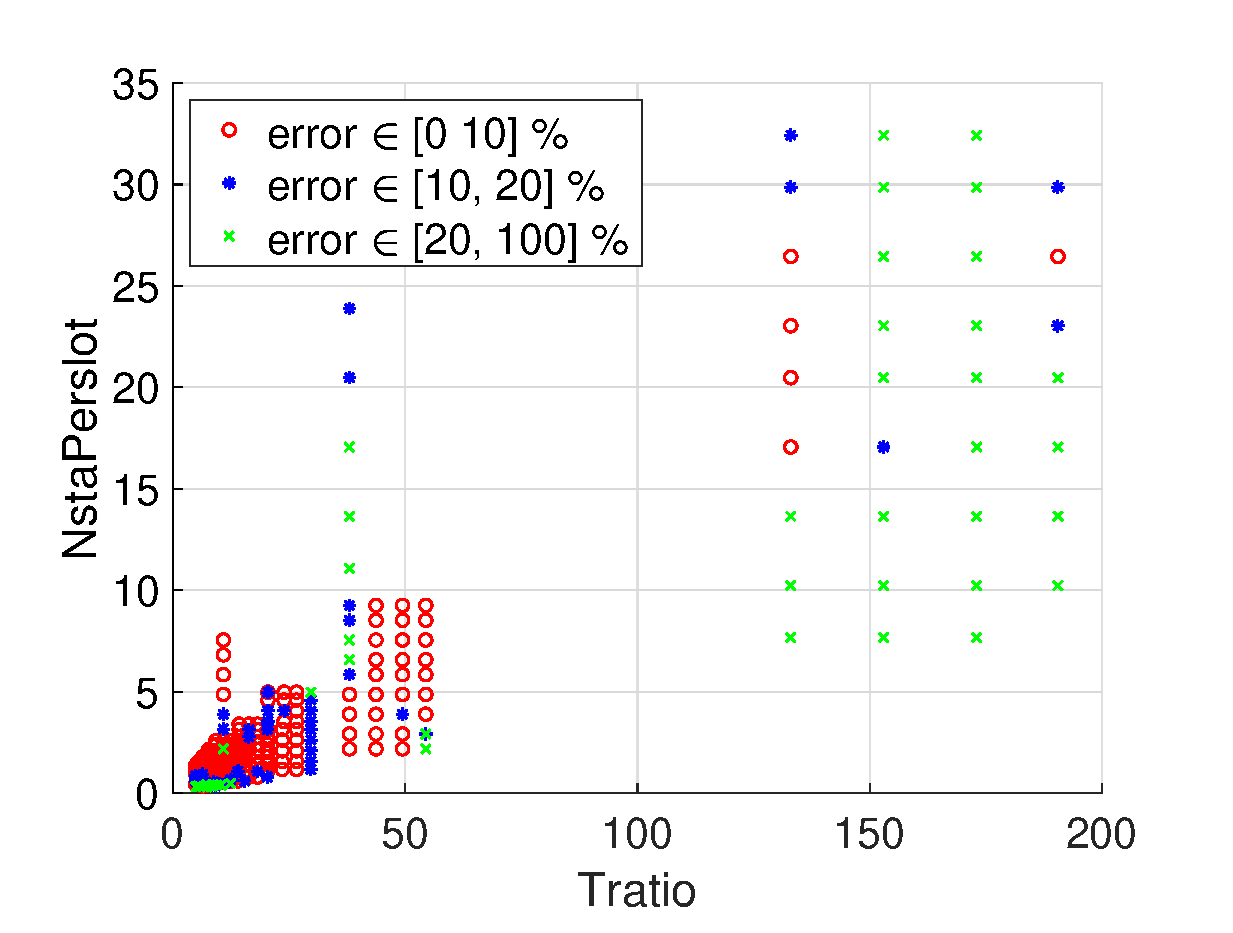
\includegraphics[width=0.33\textwidth]{figures/nstaPerSlot_Tratio_scatter_tx3000}}
    \subfloat[Tx 4000 us \label{fig:scatter_ana_tx4000}]{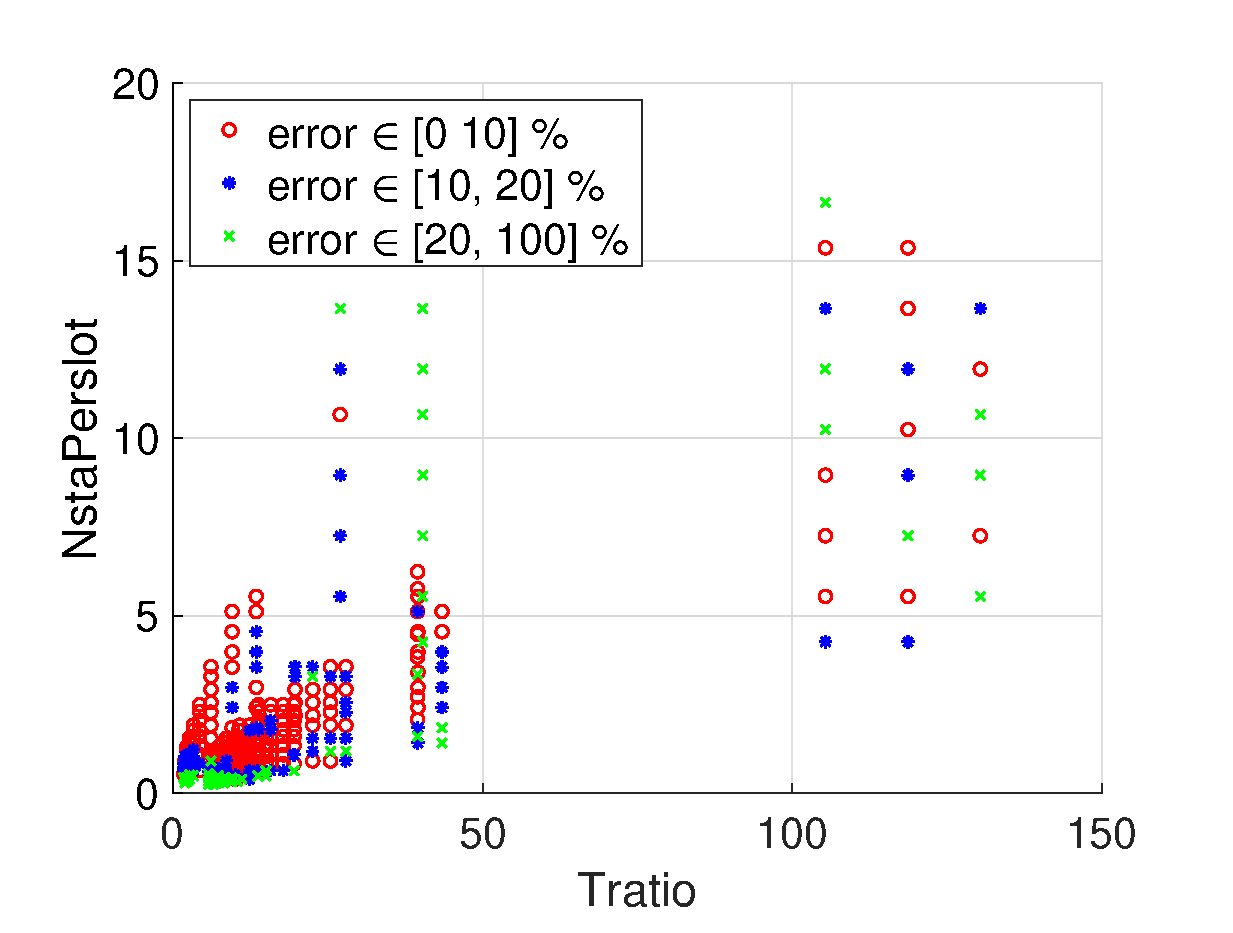
\includegraphics[width=0.33\textwidth]{figures/nstaPerSlot_Tratio_scatter_tx4000}}
    %\subfloat[Full design space with various types of transmission time \label{fig:delay-alpha-0}]{\includegraphics[width=0.33\textwidth]{figures/scatter_randomTx}}
  \caption{Illustration of the relations among model accuracy and $n^{\alpha}_r$ and  $d^{\beta}_r$. \label{fig:scatter-plot-ana}}
\end{figure*}

% \begin{figure}[t]
%     \centering
%     \subfloat[Color represents the transmission time (us)  \label{fig:delay-alpha-0}]{\includegraphics[width=0.8\columnwidth]{figures/scatter_results-error-GPR5020-opti-all-sort-3D-L0_1}} \\
%      \subfloat[Color represents the slot number  \label{fig:delay-alpha-0}]{\includegraphics[width=0.8\columnwidth]{figures/scatter_results-error-GPR5020-opti-all-sort-3D-L0_1-angle}} 
%   \caption{3D Scatter plot for Relative error $>=$ 0.1. \label{fig:3d-Scatter-plot}}
% \end{figure}


% \begin{figure}[t]
%     \centering
% {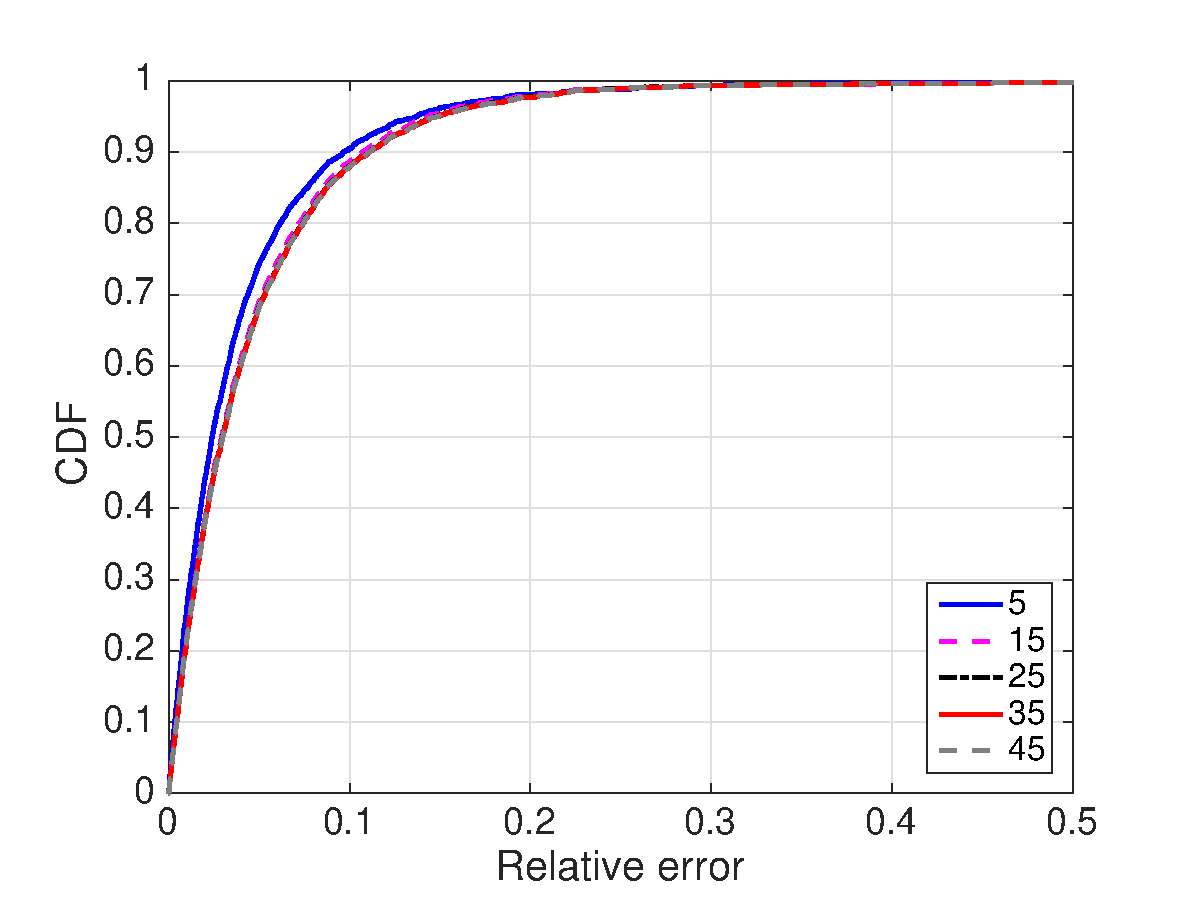
\includegraphics[width=0.8\columnwidth]{figures/cdf_all_ratio_NstaPslot_S50_Tratio_L1}}
%   \caption{Accuracy of \gls{gpr} regression model for full design space with different slot load ratio. \label{fig:cdf_constraint}}
% \end{figure}

\begin{figure}[t]
    \centering
{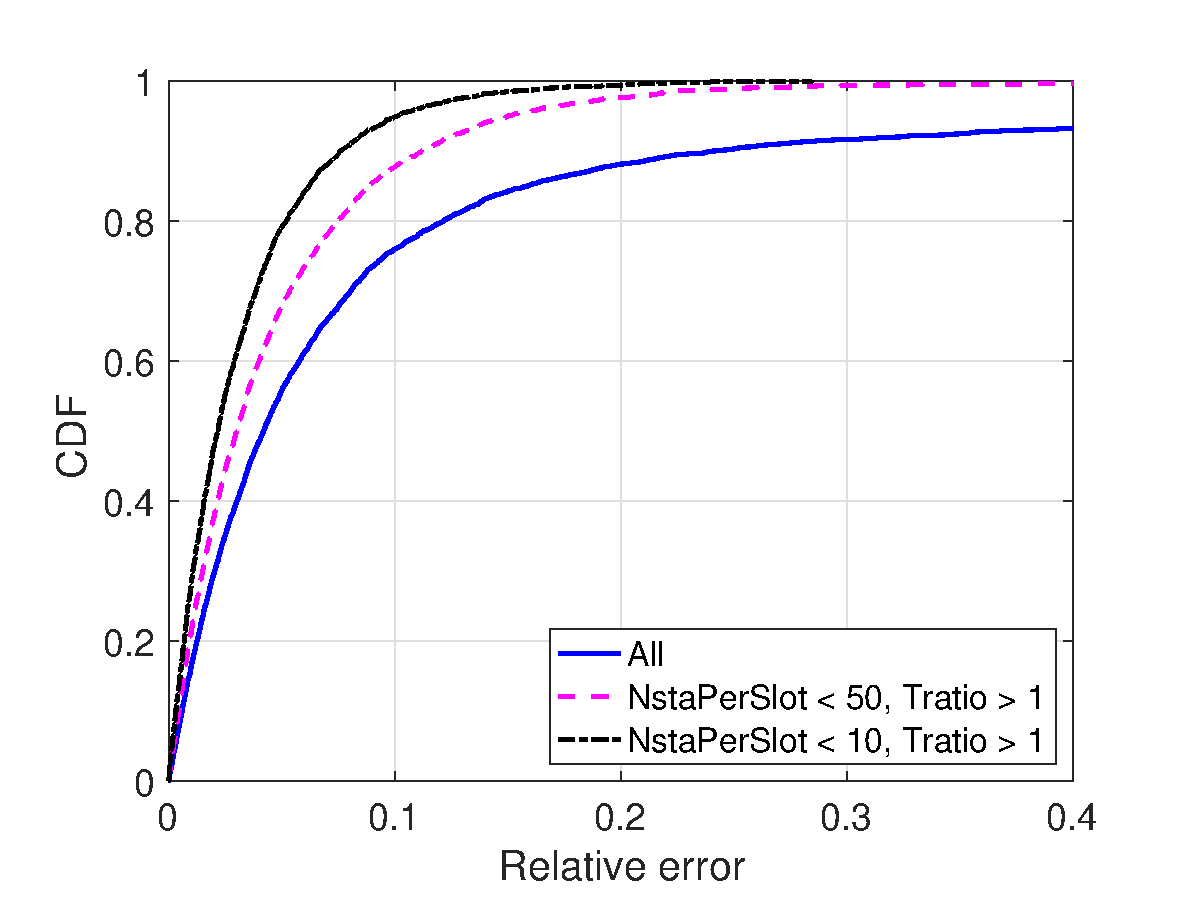
\includegraphics[width=0.8\columnwidth]{figures/full_constraint}}
  \caption{Accuracy of surrogate model using Kriging method for full design space with different constraints. \label{fig:cdf_constraint}}
\end{figure}

% \begin{figure}[t]
%     \centering
%     \subfloat[Relative error $<=$ 0.1  \label{fig:delay-alpha-0}]{\includegraphics[width=0.8\columnwidth]{figures/random_NstaPerSlot_Tratio_S01}} \\
%      \subfloat[Relative error $>$ 0.1 \label{fig:delay-alpha-0}]{\includegraphics[width=0.8\columnwidth]{figures/random_NstaPerSlot_Tratio_L01}} 
%   \caption{Distribution of station number per slot and xx for different Relative error \label{fig:3d-Scatter-plot}}
% \end{figure}


% \begin{figure}[t]
%     \centering
% {\includegraphics[width=0.8\columnwidth]{figures/cases_reduced}}
%   \caption{Accuracy of \gls{gpr} regression model for full and reduced design space. \label{fig:casess}}
% \end{figure}



% \begin{figure}[t]
%     \centering
% {\includegraphics[width=0.8\columnwidth]{figures/cases_randomTx}}
%   \caption{Accuracy of \gls{gpr} regression model for full design space with various types of transmission time. \label{fig:cases_randomTx}}
% \end{figure}


% \begin{figure}[t]
%     \centering
% {\includegraphics[width=0.8\columnwidth]{figures/sim-compare-rd204800-sl10}}
%   \caption{Comparison of simulation results for transmission time (2000 us) with different distance range of packet size range . \label{fig:tx_diff_compare}}
% \end{figure}



% \begin{figure}[t]
%     \centering
% {\includegraphics[width=0.8\columnwidth]{figures/same_diff}}
%   \caption{Accuracy of \gls{gpr} regression model for same and different MCS and packet size (reduced design space). \label{fig:cases_reduced}}
% \end{figure}

% \begin{figure*}[t]
%     \centering
%     \subfloat[same \label{fig:delay-alpha-0}]{\includegraphics[width=0.45\textwidth]{figures/same_sim_model_scatter}}
%     \subfloat[diff \label{fig:delay-alpha-0}]{\includegraphics[width=0.45\textwidth]{figures/diff_sim_model_scatter}}
%   \caption{Scatter plot. \label{fig:scatter-plot-tx}}
% \end{figure*}

% \begin{figure}[t]
%     \centering
% {\includegraphics[width=0.8\columnwidth]{figures/seed_sim_model_scatter}}
%   \caption{Comparison between simulation results using different seed . \label{fig:seed-comparison}}
% \end{figure}


% \begin{figure}[t]
%     \centering
% {\includegraphics[width=0.8\columnwidth]{figures/result-rd204800-pslot}}
%   \caption{comparison between model and simulation with * stations per slots. \label{fig:staPerSlot}}
% \end{figure}

In this section, we evaluate the \gls{raw} model accuracy for the limited design space, in which the average transmission time consists of the coverage and packet size ranges used during the training process. As the design space includes xx data points, it is extremely expensive to run all experiments. Therefore, 6000 data points (called test data points) are randomly chosen for the evaluation of the model. To evaluate the accuracy of kriging model (with Matem 5/2) used in the model creation step, three additional regression models (i.e., linear regression, \gls{svm} and regression trees) are also created with the trained data points for comparison. The simulation results of the 6000 test data points are compared to the prediction of the models. 


% Figure \ref{fig:regress-models} depicts the probability that the relative error (i.e., ratio between absolute throughput error and simulation results) of the  models compared to simulation are equal to or less than a given relative error.

Figure \ref{fig:regress-models} depicts the \gls{cdf} of the relative error, i.e., ratio \textcolor{red}{between absolute throughput error of the model and simulation,  and simulation results}.
It shows 76\% of the test data points has a relative error equal to or less than 0.1 for kriging model with Matem 5/2, while 30\%, 10\% and 44\% for the linear regression, \gls{svm}, regression tree models respectively. Similarly,  for kriging model, 88\% of the test data points result in  a relative error not larger than 0.2, the percentage declines to 53\%, 17\% and 65\% for the linear regression, \gls{svm} and regression tree models respectively. The results show the Kriging model has higher accuracy than the other three regression models. However, there are still some data points with high relative error and we will further investigate. 
%the model is not good enough to be directly applied to the \gls{raw} modeling problem. %\textcolor{red}{consider to remove the line of Kriging, Matem 3/2}.


To further explore the performance of the Kriging model, Figure \ref{fig:scatter-plot}  shows a scatterplot of the output of simulation and predication of the model.
%for the same test data points.
The line  $y=x$ represents the ideal case where the model can precisely predict the output of all data points without any errors. Points located near the line $y=x$ indicates that they can be accurately predicated by the model, and vice versa. The points are color-coded based on the relative errors, red means the relative error lower than 10\%, blue represent the relative error between 10\% and 20\%, and green indicates the error larger than 20\%. Figure \ref{fig:scatter_all} reveals interesting characteristic of the created \gls{raw} model, the large error mainly exists for the small packet rates, which makes sense as a small absolute error leads to a large relative error. As the model is mainly used for \gls{raw} optimization, we are more interested in the large values, as these signify higher throughput and better performance. \textcolor{red}{Most of the points} with relative error between 10\% and 20\%  have packet rate below 150, \textcolor{red}{most of the relative error} larger than 20\% appear when the packet rate is below 100, large errors are especially concentrated at packet rates below \textcolor{red}{40}. 

Moreover, the relative error varies for points with different average transmission times. Figure \ref{fig:full_design_error} depicts the relative error as a function of the packet receiving rate (simulation result) with transmission time $1000$, $2000$, $3000$ and $4000$ us respectively. Similar to figure  \ref{fig:scatter_all}, it shows the high relative error mainly exists for low packet receiving rate. Moreover, the results reveals the smaller average transmission time results in less relative error than larger average transmission.
 
%  Compare to transmission time $4000$ \textit{us}, the transmission time $1000$ \textit{us} results in much less error, there is a few points with error between 10\% and 20\%, and errors beyond 20\% (\textcolor{red}{the figure needs to be replotted}). While transmission time $4000$ \textit{us} has the similar error distribution as figure \ref{fig:scatter_all}. In addition, for the same packet rate, transmission time $1000$ \textit{us} results in less error than $4000$ \textit{us} does. For example, it has much less points with error between 10\% and 20\% in the packet rate range [50, 150].


% Take $1000$ and $4000$ \textit{us} as an example, figure \ref{fig:scatter_tx1000} and \ref{fig:scatter_tx4000} depict the scatterplot for points with transmission time $1000$ and $4000$ \textit{us} respectively. Compare to transmission time $4000$ \textit{us}, the transmission time $1000$ \textit{us} results in much less error, there is a few points with error between 10\% and 20\%, and errors beyond 20\% (\textcolor{red}{the figure needs to be replotted}). While transmission time $4000$ \textit{us} has the similar error distribution as figure \ref{fig:scatter_all}. In addition, for the same packet rate, transmission time $1000$ \textit{us} results in less error than $4000$ \textit{us} does. For example, it has much less points with error between 10\% and 20\% in the packet rate range [50, 150].

In conclusion, from figure \ref{fig:scatter-plot}, we discover that, for the design space, the surrogate \gls{raw} model model can accurately predict the output when the packet receiving rate is high, which is vital for the \gls{raw} model as it is commonly used for maximizing the packet receiving rate (equivalent to high throughput). Therefore, the model can actually be applied to the \gls{raw} modeling problem if the data points resulting in low packet rate are excluded from the model.
%Last but not least, the output (packet rate) of data point with high transmission time has higher variance.

% \textcolor{red}{Two question of figure \ref{fig:regress-models}:} \\
% \textcolor{red}{Should CDF of relative error be used or cross validation score?} \\
% \textcolor{red}{Should a random test data set or the training data set be used?} \\
%\item Measure accuracy in all cases, find weaknesses in the model. \\
 
 
%As the goal of \gls{raw} is to maximize the throughput (packet receiving rate) in dense scenarios with heavy traffic load, the \gls{raw} configurations that result in low packet rate can be excluded from the model, allowing the model to accurately predict the output of the given \gls{raw} configuration.
 
 %Let $NstaPSlot$ denote the number of stations per \gls{raw} slot, and $Tratio$ represent the ratio between \gls{raw} slot duration and transmission time.
Figure \ref{fig:scatter-plot-ana} shows the scatterplot of the number of stations in one \gls{raw} slot ($N^{\alpha}_{r}$) and the ratio between \gls{raw} slot duration and transmission time ($N^{\beta}_r$), for different relative errors. As it reveals, for transmission times $3000$ and $4000$ \textit{us}, the larger errors mainly exist for \gls{raw} configuration in which either too many stations contend for the channel in one \gls{raw} slot or the \gls{raw} slot duration is too short to transmit one packet, resulting in low packet rate \textcolor{red}{(not depicted)}. Therefore, to accurately predict the output of a given \gls{raw} configuration, a constraint is added when applying the model, i.e., 
\begin{equation} \label{eq:constraint}
n^{\alpha}_r < \alpha \wedge d^{\beta}_r >= \beta
\end{equation}
% Through analyzing the simulation results and model, we found out that the low packet rate are mainly caused by the inefficient \gls{raw} configurations, either too much stations contending the channel in one raw slot or the raw slot duration is too short to transmit one packet. 
%\item Go to more realistic cases at the end of this section, where the results are better. (for reduced and full design space, to compare the difference in performance) \\
Therefore, the \gls{cdf} of the relative error for the Kriging model is updated with different $\alpha$ and $\beta$, and depicted in Figure \ref{fig:cdf_constraint}. As it shows, nearly 90\% of the data points have a relative error equal to or less than 0.1 for $\alpha = 50$ and $\beta = 1$. If $\alpha$ is further reduced to 10, the percentage goes up to 95\%. 





% Figure \ref{fig:casess} shows the accuracy of \gls{gpr} regression model under different cases. 
% The performance of model accuracy between reduced and full design space is compared. \\
% \textcolor{red}{what kind of data set should be used for comparison? \\
% \begin{enumerate}
% \item data set including points inside and outside of the reduced design space?
% \item or two different data set? one is inside, another one is outside.
% \end{enumerate}
%}

\subsection{\textcolor{red}{Extrapolated design space experiments}}

% \begin{figure*}[t]
%     \centering
%     \subfloat[tx1000 204800 \label{fig:tx_diff_tx1000}]{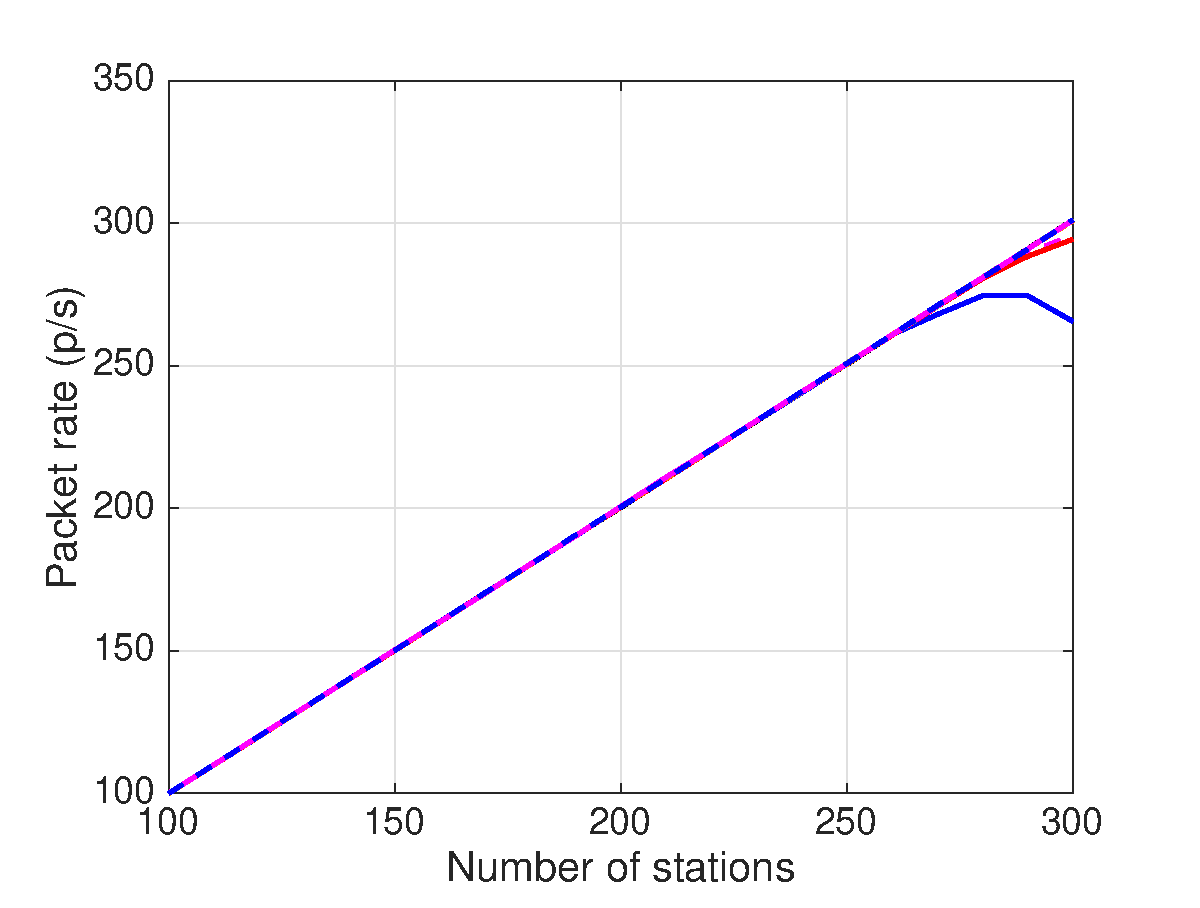
\includegraphics[width=0.45\textwidth]{figures/tx1000_204800}}
%     \subfloat[tx5000 204800 \label{fig:tx_diff_tx5000}]{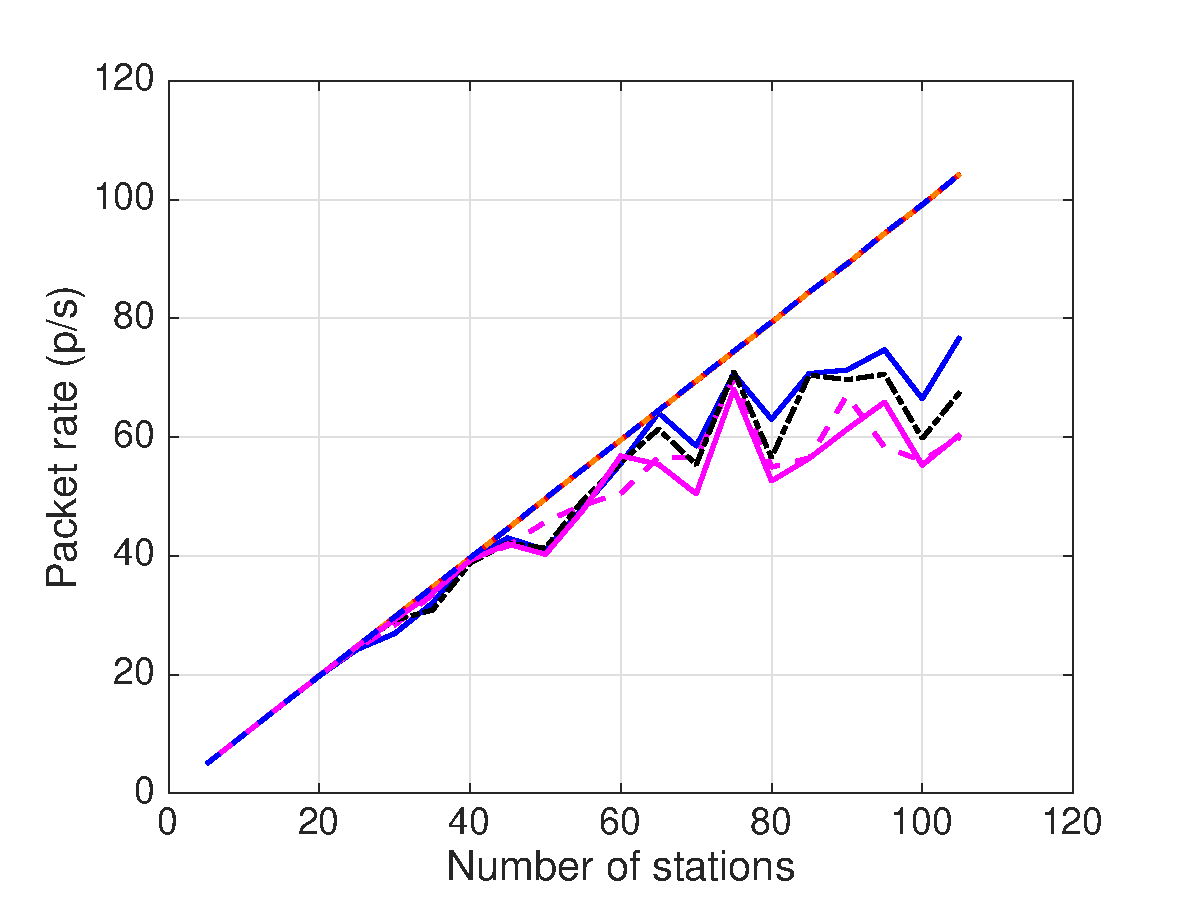
\includegraphics[width=0.45\textwidth]{figures/tx5000_204800}}
%   \caption{Comparison of simulation results for transmission time (2000 us) with different distance range of packet size range. \label{fig:tx_diff_compare}}
% \end{figure*}

%  One of the input parameters used by the \gls{raw} modeling, \textit{average transmission time}, is actually represented by two parameters of the 802.11ah network, i.e., distance between stations and \gls{ap}, and packet size of the stations. In the modeling process, for each average transmission time, the network are configured with a fixed distance range and packet size. However, there are a large number of distance and packet size range that can lead to the same average transmission time. 
 
 The results in previous section have demonstrated that, under certain constraints, the built model has high accuracy on predicting the output for the design space. In this section, we further explore the performance of the model for the extrapolated design space. In the extrapolated design space, 
 a data point with average transmission time Tx, consists of different coverage and packet size ranges than the one used during the training.
 
 
 \begin{figure}[t]
    \centering
{\includegraphics[width=0.8\columnwidth]{figures/Extend_constraint}}
  \caption{Accuracy of Surrogate model using Kriging method for extrapolated design space with different constraints. \label{fig:cdf_constraint_extended}}
\end{figure}
 
The 6000 test data points used in Figure \ref{fig:regress-models} and Figure \ref{fig:cdf_constraint} are again simulated. However, for a data point with average transmission time Tx, the simulator randomly selects a  coverage and packet size range which can result in the average transmission time Tx. The simulation results are compared to the output of the built models, as shown in Figure \ref{fig:cdf_constraint_extended}. It shows, compare to the limited design space, the extrapolated design space results in more error in terms of model accuracy. Even under the constraint $n^{\alpha}_r < 10 \wedge d^{\beta}_r >= 1$, the model accuracy is still not satisfying. Around 60\% of data points have relative error less than 10\%. The number goes up to 78\% for a relative error less than 20\%. The lower model accuracy for the extrapolated design space is not surprising. In the modeling process, for each average transmission time, the network is configured with a fixed distance range and packet size. However, in the extrapolated design space, for the same average transmission time, the network could could be configured with other distance  and packet size ranges. Therefore, model accuracy is sacrificed in order to speed up the training process. This aligns with our discovery in Section \ref{subsubsec:txselection}, which also indicates high model accuracy can still be achieved for the scenarios that we are interested in, \todo{explain the scenarios}. 
 
%  In order to make the trained model more applicable to the extrapolated design space, we first explore the performance difference of a variety of distance and packet size range leading to the same average transmission time. For each data point, 10 different distance and packet size range are randomly selected and simulated. Take average transmission time  $1000$ and $5000$ us as an example, figure \ref{fig:tx_diff_compare} shows, the packet receiving rate as a function of station number for \gls{raw} duration $204800$ \textit{us} and slot number $10$. The lines represent the 10 different iterations. The result shows that the same packet rate is achieved until a certain number of stations, then discrepancy among the packet rates of different distance and packet size ranges starts to appear. Moreover, the breaking points where the discrepancy occurs depends on the average transmission time. As figure \ref{fig:tx_diff_tx1000} shows, the packet rate start to vary when station number is 260, while the performance difference is triggered by much less stations (around 45) fro transmission time $5000$ \textit{us}.  With a given slot number and \gls{raw} duration, station number determines the traffic load of the \gls{raw} slot. Therefore, figure \ref{fig:tx_diff_compare} indicates that, the performance discrepancy is caused by the  high traffic load $L_r$:  \\
% \begin{equation}
% \mathcal{L}_{r} = \frac {n_r \times TXOP} {d_r \times \mathcal{T}_s}.
% \end{equation}
% Where $TXOP$ indicate the TXOP time including data packet transmission time ($T_x$), a SIFS (160 us) and the ACK transmission time (1000 us), $\mathcal{T}_s$ represents the packet sending interval of a station. The minimal slot traffic load which can cause performance discrepancy is denoted as $\mathcal{L}_r^max$, in order to apply the model to the extended design space, the slot traffic load needs to be no larger than the $\mathcal{L}_r^max$.
% For transmission time $1000$ and $5000$ \textit{us}, the  $\mathcal{L}_r^max$ are \textcolor{red}{xx} and \textcolor{red}{xx}, respectively. %As the DIFS and backoff time is not taken into account, 


To further evaluate the model accuracy, We randomly choose 500 design points for each load ratio (i.e., 0.4, 0.6, 0.8, 1.0 and 1.6), consisting of 5 different average transmission time (i.e., 1000, 2000, 3000, 4000 and 5000 us). During simulation, for each design point, the network is configured with a randomly coverage and packet size range, while satisfying the average transmission time $T_x$. Each simulation runs for 10 times.
%with the variability of result over these iterations quantified using the standard deviation (SD).
Under the constraint indicated in equation \ref{eq:constraint} with $\alpha=10$ and $\beta=1$, the relative error of each design point between the simulation results and the surrogate model is calculated. For each average transmission time, the relative error is averaged among data points with the same packet receiving rate and slot load ratio respectively. Furthermore, the relative error is averaged among all iterations, as depicted in figure \ref{fig:results-extended-prate}   and \ref{fig:results-extended-load} respectively . 

The results show, for the extrapolated design space, the surrogate model is able to accurately predict the network performance for most of the scenarios. As depicted in Figure \ref{fig:results-extended-prate}, the relative error increases with higher average transmission time. Moreover, the small packet receiving rate (less than or equal to 50) results in high relative error, while small relative error is obtained for larger packet receiving rates. By excluding the data points with the packet receiving rate less than or equal to 50, figure \ref{fig:results-extended-load} further reveals the model accuracy varies on the \gls{raw} slot load. For average transmission time 1000 us, the relative error is only 0.38\% for slot load ratio 0.4, and increase to 7.6\% for overloaded traffic (i.e., slot load ratio 1.6\%). Average transmission time 2000, 3000 and 4000 us have similar relative errors \textcolor{red}{from slot load ratio 0.4 and 1.0} (i.e., non saturated traffic conditions), ranging from 3.6\% to 14.1\%. While for average transmission time 5000 us, the relative error is already 23.4\% for slot load ratio 1, and increases to 53.5\% for slot load ratio 1.6.

%\textcolor{red}{analysis of optimal raw duration and slot number for a given station number and average transmission time.}


% \begin{figure}[t]
%     \centering
% {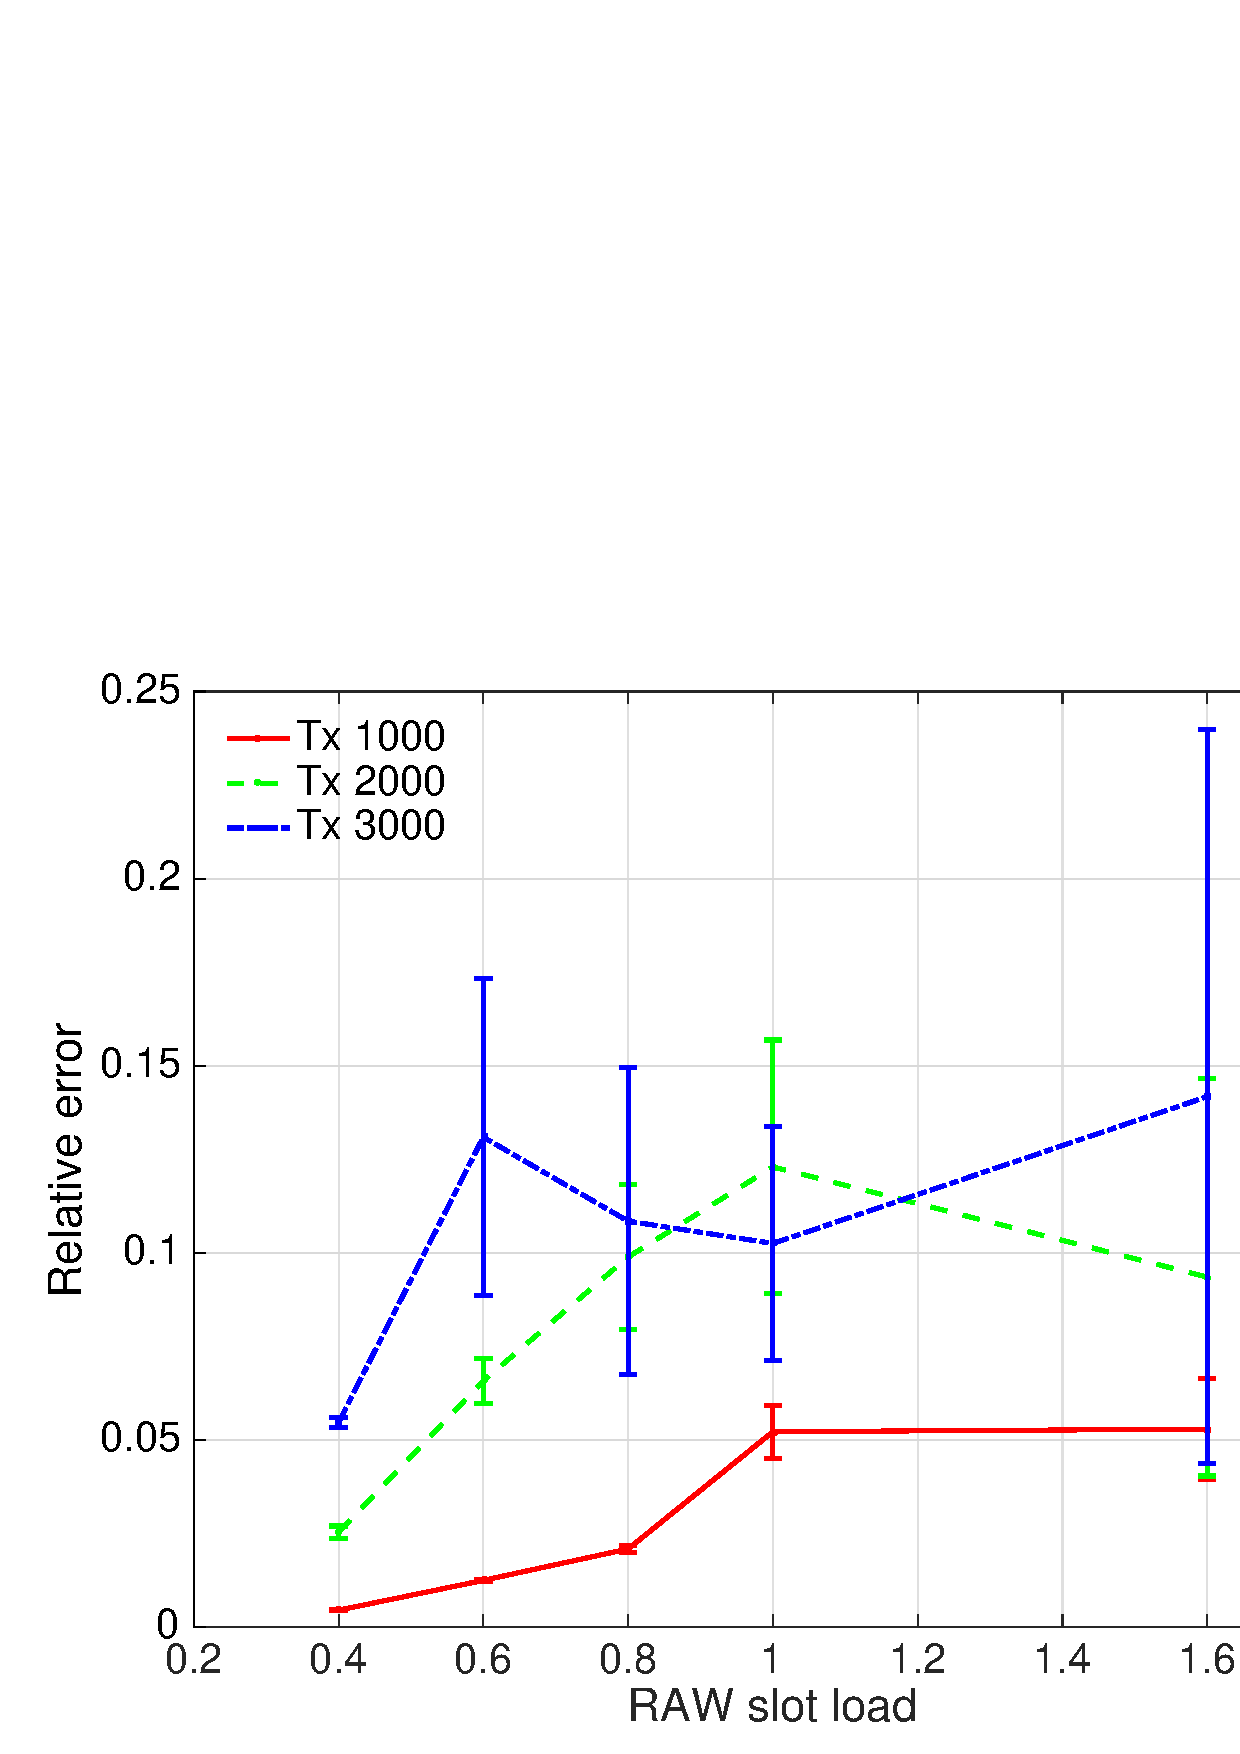
\includegraphics[width=0.8\columnwidth]{figures/1_50_tx3000.pdf}}
%   \caption{Performance for extended design space with different slot load ratio and average transmission time. \label{fig:results-extended}}
% \end{figure}



% \begin{figure*}[t]
%     \centering
%     \subfloat[Tx 1000-4000 us  \label{fig:tx_diff_tx1000}]{\includegraphics[width=0.45\textwidth]{figures/1_50_error_toTx4000.pdf}}
%     \subfloat[Tx 4000-5000 us  \label{fig:tx_diff_tx5000}]{\includegraphics[width=0.45\textwidth]{figures/1_50_error_toTx5000.pdf}}
%   \caption{Performance for extrapolated design space with different slot load ratio and average transmission time. \textcolor{red}{to be merged}   \label{fig:results-extended-load}}
%   % not fliter out small output
% \end{figure*}

 \begin{figure}[t]
    \centering
{\includegraphics[width=0.8\columnwidth]{figures/tx_result_load_all_yxlim}}
  \caption{Performance for extrapolated design space with different packet receiving rate and average transmission time. \label{fig:results-extended-prate}}
  % new load ratio, from 2-8
\end{figure}


 \begin{figure}[t]
    \centering
{\includegraphics[width=0.8\columnwidth]{figures/1_50_error_fliter}}
  \caption{Performance for extrapolated design space with different slot load ratio and average transmission time. \label{fig:results-extended-load}}
  % new load ratio, from 2-8, fliter out small output
\end{figure}


% \begin{figure*}[t]
%     \centering
%     \subfloat[Tx 1000-3000 us  \label{fig:tx_diff_tx1000}]{\includegraphics[width=0.45\textwidth]{figures/tx_1_3000.pdf}}
%     \subfloat[Tx 4000-5000 us  \label{fig:tx_diff_tx5000}]{\includegraphics[width=0.45\textwidth]{figures/tx_1_4_5000.pdf}}
%   \caption{Performance for extrapolated design space with different slot load ratio and average transmission time. \label{fig:results-extended}}
% \end{figure*}






%As the ns-3 based 802.11ah simulator provides a quite realistic simulation environment, in which the propagation loss, capture effect are considered, the distribution of distance (Equivalent to MCS) and packet size imposes an impact on the channel contention and thus affect the packet rate.


% The figure \ref{fig:cases_reduced} compares the model accuracy for both reduced and full design space under realistic cases. A random test including xx data points belonging to the full design space was simulated and the results are compared to the  models of reduced and full design space. When compared to the reduced design space, for the data points outside of the design space, we choose the output of the closest data points inside the reduced design space as its approximation. Therefore, in fact, the model for the reduced design space (figure \ref{fig:cases_reduced}) is a Interpolation.

% \item Same MCS and packet size
% \begin{itemize}
% \item CDF of relative error.
% \item Scatter plot
% \item Compare model and simulation results.
% \end{itemize}

% \item Different MCS and packet size
% \begin{itemize}
% \item Comparison of regression models
% \item CDF of relative error, graphs with different constraints can be shown.
% \item Compare model and simulation results.
% %\item Compare model and simulation results, number of staitons per slot.
% \end{itemize}

%\item plot ''accuracy = Tsim (RDm, SLm) / Tsim (RDs, SLs)" 
%\textcolor{red}{The test data set needs to be large enough, otherwise the accuracy could be much larger than 1.}

%\item throughput comparison
%\item analysis of optimal raw duration and slot number for a given station number and average transmission time.
%\end{itemize}



\subsection{Exploring optimal \gls{raw} configuration}

%\textcolor{red}{analysis of optimal raw duration and slot number for a given station number and average transmission time.}

We evaluate the scenarios in which stations are randomly located around the \gls{ap} with distance no more than 500 meters, and have packet size between 64 and 512 bytes. The average transmission time of such networks are around 2000 us. Figures \ref{fig:result-rd} compares the surrogate model and simulation results under different stations number, slot number and \gls{raw} duration. The lines represents the simulation results, and the the dots represent the  model prediction. As it shows, the simulation results and the model predictions are quite close in most cases, and most importantly, always have the same trend. As it shows, the large \gls{raw} duration normally leads to higher packet rate, which is straightforward as there is more airtime for packet transmission. While too long \gls{raw} duration is a waste of airtime, as stations not belonging to the \gls{raw} group can not access the channel. The appropriate \gls{raw} duration should be just long enough for transmitting all the packets. For a given \gls{raw} duration, too many station could degrade the performance as too much collision occurs.
It turns out a large number of \gls{raw} slot often leads to better performance, especially for large scale networks.

% A better way to assess and apply the model is needed based on the following observations.
% \begin{itemize}
% \item The simulation results fluctuates with station number.
% \item The simulation results and model have the same trend, but their actual values could be different.
% \item Under average transmission time 2000 us, the optimal configuration (i.e., slot number) for a given station number and \gls{raw} duration are same for both model and simulation results. 
% \end{itemize}

% Figures \ref{fig:result-slot} 
% compares model and simulations results with fixed average transmission time duration under different stations number, slot number and \gls{raw} duration.

% A better way to assess and apply the model is needed based on the following observations.
% \begin{itemize}
% \item The simulation results fluctuates with station number, especially for the large distance range (i.e., 0~400 m and 0~500 meters).
% \item The simulation results and model have the same trend.
% \item The simulation results and model are close until a certain point (throughput/station number).
% \item The optimal configuration (i.e., slot number) for a given station number and \gls{raw} duration are same for both model and simulation results. 
% \end{itemize}

% \textbf{Although the absolute output of the model and simulation does not match, they have the same trend, which is crucial in the selection of optimal \gls{raw} configuration under a given station number and average transmission time. especially for the scenarios whose distance and packet size range are different from the trained scenarios.}

% The difference between model and results with 0-100 meters and slot 10/20, 0-300 m and slot 10, is caused by the average transmission time distribution. Due to the non cross slot boundary transmission features, packet has different chance to transmit during its own slot. 




\begin{figure*}[t]
    \centering
    \subfloat[rd = 122880 us  \label{fig:delay-alpha-0}]{\includegraphics[width=0.33\textwidth]{figures/result-rd122880}}
    \subfloat[rd = 163840 us \label{fig:delay-alpha-0}]{\includegraphics[width=0.33\textwidth]{figures/result-rd163840}}
     \subfloat[rd = 204800 us \label{fig:delay-alpha-0}]{\includegraphics[width=0.33\textwidth]{figures/result-rd204800}}
  \caption{Comparison between model and simulations results with fixed average transmission time (2000 us) under different stations number, slot number and \gls{raw} duration.  \label{fig:result-rd}}
\end{figure*}


% \begin{figure*}[t]
%     \centering
%     \subfloat[ 0-100 m \label{fig:delay-alpha-0}]{\includegraphics[width=0.33\textwidth]{figures/result-rd204800-range100}}
%     \subfloat[ 0-300 m \label{fig:delay-alpha-0}]{\includegraphics[width=0.33\textwidth]{figures/result-rd204800-range300}}
%      \subfloat[0-400 m \label{fig:delay-alpha-0}]{\includegraphics[width=0.33\textwidth]{figures/result-rd204800-range400}}
%   \caption{Comparison between model and simulations results with fixed \gls{raw} duration (204800 us) under different stations number, slot number, distance range (transmission time).   \label{fig:result-range}}
% \end{figure*}

% \begin{figure*}[t]
%     \centering
%     \subfloat[ rd = 163840 us, 0-400 m \label{fig:delay-alpha-0}]{\includegraphics[width=0.45\textwidth]{figures/NstaPSlot-result-rd163840-range400}}
%      \subfloat[ rd = 204800 us, 0-500 m \label{fig:delay-alpha-0}]{\includegraphics[width=0.45\textwidth]{figures/NstaPSlot-result-rd204800-range500}}
%   \caption{Comparison between model and simulations results under different stations number, number of stations per slot, distance range.   \label{fig:result-slot}}
% \end{figure*}

% \begin{figure*}[t]
%     \centering
%     \subfloat[ 0-300 m \label{fig:delay-alpha-0}]{\includegraphics[width=0.45\textwidth]{figures/NstaPSlot-Thr-result-rd163840-range400}}
%      \subfloat[ 0-100 m \label{fig:delay-alpha-0}]{\includegraphics[width=0.45\textwidth]{figures/NstaPSlot-Thr-result-rd204800-range500}}
%   \caption{Comparison between model and simulations results with fixed \gls{raw} duration under different stations number, slot number, distance range.   \label{fig:result-slot-throughput}}
% \end{figure*}



% There are two ways to interpret the results.

% The first one is, model can accurately predicts the output for practical scenarios, i.e., \gls{raw} duration is at least one/two times larger than average transmission time (one for trained transmission time, two for any transmission time composition), and no more than 10 stations assigned per slot. The downside is, some \gls{raw} configuration whose output can be very well  predicted are excluded from the practical scenarios". Figures like Figure \ref{fig:result-rd} and \ref{fig:result-range} can not be shown. One more question is also aroused, does the practical scenarios" includes the optimal \gls{raw} configuration for any given station number and transmission time. 

% Figures/table needed:
% \begin{itemize}
% \item large relative error only exist for small output (option, only suitable for the trained scenarios, this can be caused by the applied machine learning model(kriging model in this case). This figure can be used to reveal/present the drawback(?) of the kriging model.   (Note:the reduced design space and full design space have quite same performance.)
% \item scatter plot, highlight the \gls{raw} configuration that result in high relative error, and leads to the 
% \item figures for constrained \gls{raw} configuration, including both design space reduced, full design space. \\
% \textcolor{red}{figure \ref{fig:result-rd}, \ref{fig:result-range} can not be used due to the constraint, but results are actually quite good. There are two reasons, first, the constraints excludes some \gls{raw} configuration which has good performance, second, the results can still be good in some case even when the accuracy" is not high (figure \ref{fig:result-rd} has relative error 0.1 for 70\% data points.)}
% \item  simulation results comparison between trained and untrained scenarios.
% \item  Accuracy of untrained scenarios with refined constraints. 
% \end{itemize}

% Another option is, do not look at the absolute output of the model and simulation, but focus on the trend, they offer the same optimal \gls{raw} configuration.








